
%% gnuplot の test

\documentclass[10pt,b5paper,papersize,dvipdfmx]{jsbook}

\usepackage{../../../sty/vuccaken}
% \usepackage[analog]{vuccaken}
% \usepackage{v-hyperref}
\usepackage{../../../sty/vuccaken2019}

\usepackage{newtxtext,newtxmath}

%% font -> gt & sf
\renewcommand\kanjifamilydefault{\gtdefault}
\renewcommand\familydefault{\sfdefault}


\usepackage{gnuplot-lua-tikz}

%
\begin{document}
%

\begin{figure}[th] \small
  \centering
  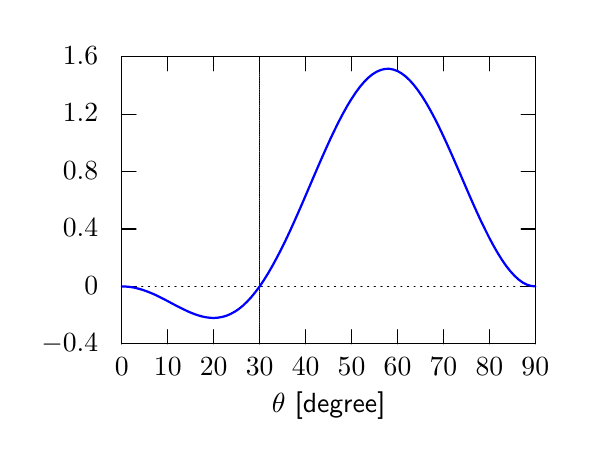
\begin{tikzpicture}[gnuplot]
%% generated with GNUPLOT 5.1p0 (Lua 5.3; terminal rev. 99, script rev. 100)
%% 月  9/23 01:31:47 2019
\path (0.000,0.000) rectangle (7.000,5.000);
\gpcolor{color=gp lt color border}
\gpsetlinetype{gp lt border}
\gpsetdashtype{gp dt solid}
\gpsetlinewidth{1.00}
\draw[gp path] (1.196,0.985)--(1.376,0.985);
\draw[gp path] (6.447,0.985)--(6.267,0.985);
\node[gp node right] at (1.012,0.985) {$-0.4$};
\draw[gp path] (1.196,1.714)--(1.376,1.714);
\draw[gp path] (6.447,1.714)--(6.267,1.714);
\node[gp node right] at (1.012,1.714) {$0$};
\draw[gp path] (1.196,2.443)--(1.376,2.443);
\draw[gp path] (6.447,2.443)--(6.267,2.443);
\node[gp node right] at (1.012,2.443) {$0.4$};
\draw[gp path] (1.196,3.173)--(1.376,3.173);
\draw[gp path] (6.447,3.173)--(6.267,3.173);
\node[gp node right] at (1.012,3.173) {$0.8$};
\draw[gp path] (1.196,3.902)--(1.376,3.902);
\draw[gp path] (6.447,3.902)--(6.267,3.902);
\node[gp node right] at (1.012,3.902) {$1.2$};
\draw[gp path] (1.196,4.631)--(1.376,4.631);
\draw[gp path] (6.447,4.631)--(6.267,4.631);
\node[gp node right] at (1.012,4.631) {$1.6$};
\draw[gp path] (1.196,0.985)--(1.196,1.165);
\draw[gp path] (1.196,4.631)--(1.196,4.451);
\node[gp node center] at (1.196,0.677) {$0$};
\draw[gp path] (1.779,0.985)--(1.779,1.165);
\draw[gp path] (1.779,4.631)--(1.779,4.451);
\node[gp node center] at (1.779,0.677) {$10$};
\draw[gp path] (2.363,0.985)--(2.363,1.165);
\draw[gp path] (2.363,4.631)--(2.363,4.451);
\node[gp node center] at (2.363,0.677) {$20$};
\draw[gp path] (2.946,0.985)--(2.946,1.165);
\draw[gp path] (2.946,4.631)--(2.946,4.451);
\node[gp node center] at (2.946,0.677) {$30$};
\draw[gp path] (3.530,0.985)--(3.530,1.165);
\draw[gp path] (3.530,4.631)--(3.530,4.451);
\node[gp node center] at (3.530,0.677) {$40$};
\draw[gp path] (4.113,0.985)--(4.113,1.165);
\draw[gp path] (4.113,4.631)--(4.113,4.451);
\node[gp node center] at (4.113,0.677) {$50$};
\draw[gp path] (4.697,0.985)--(4.697,1.165);
\draw[gp path] (4.697,4.631)--(4.697,4.451);
\node[gp node center] at (4.697,0.677) {$60$};
\draw[gp path] (5.280,0.985)--(5.280,1.165);
\draw[gp path] (5.280,4.631)--(5.280,4.451);
\node[gp node center] at (5.280,0.677) {$70$};
\draw[gp path] (5.864,0.985)--(5.864,1.165);
\draw[gp path] (5.864,4.631)--(5.864,4.451);
\node[gp node center] at (5.864,0.677) {$80$};
\draw[gp path] (6.447,0.985)--(6.447,1.165);
\draw[gp path] (6.447,4.631)--(6.447,4.451);
\node[gp node center] at (6.447,0.677) {$90$};
\gpsetlinetype{gp lt axes}
\gpsetdashtype{gp dt axes}
\draw[gp path] (1.196,1.714)--(6.447,1.714);
\draw[gp path] (1.196,0.985)--(1.196,4.631);
\gpsetlinetype{gp lt border}
\gpsetdashtype{gp dt solid}
\draw[gp path] (1.196,4.631)--(1.196,0.985)--(6.447,0.985)--(6.447,4.631)--cycle;
\gpsetdashtype{dash pattern=on 1.00*\gpdashlength off 1.00*\gpdashlength }
\draw[gp path](2.946,0.985)--(2.946,4.631);
\node[gp node center] at (3.821,0.215) {$\theta$ [degree]};
\gpcolor{rgb color={0.000,0.000,1.000}}
\gpsetdashtype{gp dt solid}
\gpsetlinewidth{2.00}
\draw[gp path] (1.196,1.714)--(1.249,1.712)--(1.302,1.707)--(1.355,1.698)--(1.408,1.685)%
  --(1.461,1.670)--(1.514,1.651)--(1.567,1.630)--(1.620,1.607)--(1.673,1.581)--(1.726,1.554)%
  --(1.779,1.527)--(1.832,1.498)--(1.886,1.470)--(1.939,1.443)--(1.992,1.417)--(2.045,1.392)%
  --(2.098,1.370)--(2.151,1.351)--(2.204,1.335)--(2.257,1.323)--(2.310,1.316)--(2.363,1.313)%
  --(2.416,1.317)--(2.469,1.326)--(2.522,1.341)--(2.575,1.363)--(2.628,1.392)--(2.681,1.427)%
  --(2.734,1.470)--(2.787,1.521)--(2.840,1.578)--(2.893,1.643)--(2.946,1.714)--(2.999,1.793)%
  --(3.052,1.878)--(3.105,1.969)--(3.158,2.067)--(3.212,2.170)--(3.265,2.277)--(3.318,2.389)%
  --(3.371,2.505)--(3.424,2.624)--(3.477,2.745)--(3.530,2.868)--(3.583,2.992)--(3.636,3.116)%
  --(3.689,3.239)--(3.742,3.360)--(3.795,3.479)--(3.848,3.595)--(3.901,3.706)--(3.954,3.813)%
  --(4.007,3.914)--(4.060,4.009)--(4.113,4.096)--(4.166,4.176)--(4.219,4.248)--(4.272,4.310)%
  --(4.325,4.364)--(4.378,4.407)--(4.431,4.440)--(4.485,4.463)--(4.538,4.476)--(4.591,4.478)%
  --(4.644,4.468)--(4.697,4.449)--(4.750,4.418)--(4.803,4.378)--(4.856,4.327)--(4.909,4.267)%
  --(4.962,4.197)--(5.015,4.119)--(5.068,4.033)--(5.121,3.939)--(5.174,3.839)--(5.227,3.733)%
  --(5.280,3.621)--(5.333,3.506)--(5.386,3.387)--(5.439,3.266)--(5.492,3.144)--(5.545,3.021)%
  --(5.598,2.898)--(5.651,2.777)--(5.704,2.659)--(5.757,2.544)--(5.811,2.434)--(5.864,2.328)%
  --(5.917,2.229)--(5.970,2.137)--(6.023,2.052)--(6.076,1.975)--(6.129,1.908)--(6.182,1.850)%
  --(6.235,1.801)--(6.288,1.763)--(6.341,1.736)--(6.394,1.720)--(6.447,1.714);
\gpcolor{color=gp lt color border}
\gpsetlinewidth{1.00}
\draw[gp path] (1.196,4.631)--(1.196,0.985)--(6.447,0.985)--(6.447,4.631)--cycle;
%% coordinates of the plot area
\gpdefrectangularnode{gp plot 1}{\pgfpoint{1.196cm}{0.985cm}}{\pgfpoint{6.447cm}{4.631cm}}
\end{tikzpicture}
%% gnuplot variables

  \caption{$f(\theta) = \cos^2 3\theta + \sin^2 2\theta - \cos^2\theta$のプロット。$0 < \theta < 30^\circ$のとき$f(\theta) < 0$である。}
  \label{a}
\end{figure}











%
%%
%%%
%%%%
%%%%%
%%%%%%
%%%%%%%
%%%%%%%%
%%%%%%%%%
%%%%%%%%%%
%%%%%%%%%%%
%%%%%%%%%%%%
%%%%%%%%%%%%%
\end{document}
%%%%%%%%%%%%%
%%%%%%%%%%%%
%%%%%%%%%%%
%%%%%%%%%%
%%%%%%%%%
%%%%%%%%
%%%%%%%
%%%%%%
%%%%%
%%%%
%%%
%%
%